\documentclass[border=5pt]{standalone}
\usepackage{tikz}

\begin{document}
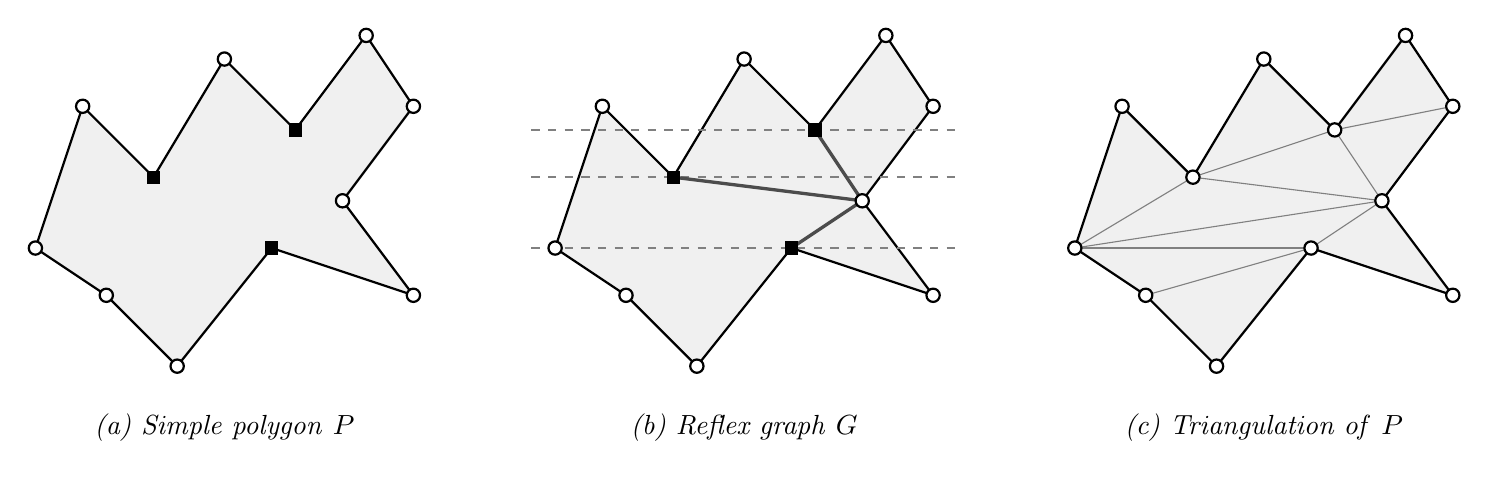
\begin{tikzpicture}[scale=0.6]

% Polygon vertices
\def\drawpoly{
    \coordinate (v0) at (0, 2.5);
    \coordinate (v1) at (1, 5.5);
    \coordinate (v2) at (2.5, 4);
    \coordinate (v3) at (4, 6.5);
    \coordinate (v4) at (5.5, 5);
    \coordinate (v5) at (7, 7);
    \coordinate (v6) at (8, 5.5);
    \coordinate (v7) at (6.5, 3.5);
    \coordinate (v8) at (8, 1.5);
    \coordinate (v9) at (5, 2.5);
    \coordinate (v10) at (3, 0);
    \coordinate (v11) at (1.5, 1.5);
}

% (a) Simple polygon P
\begin{scope}[xshift=0cm]
    \drawpoly
    \fill[gray!12] (v0)--(v1)--(v2)--(v3)--(v4)--(v5)--(v6)--(v7)--(v8)--(v9)--(v10)--(v11)--cycle;
    \draw[thick] (v0)--(v1)--(v2)--(v3)--(v4)--(v5)--(v6)--(v7)--(v8)--(v9)--(v10)--(v11)--cycle;
    
    % Convex (circles)
    \foreach \i in {0,1,3,5,6,7,8,10,11}
        {\fill[white] (v\i) circle (4pt); \draw[thick] (v\i) circle (4pt);}
    % Reflex (black squares) - split/merge vertices
    \foreach \i in {2,4,9}
        {\fill[black] (v\i) ++(-4pt,-4pt) rectangle ++(8pt,8pt);}
        
    \node[below] at (4, -0.8) {\textit{(a) Simple polygon} $P$};
\end{scope}

% (b) Reflex graph G
\begin{scope}[xshift=11cm]
    \drawpoly
    \fill[gray!12] (v0)--(v1)--(v2)--(v3)--(v4)--(v5)--(v6)--(v7)--(v8)--(v9)--(v10)--(v11)--cycle;
    \draw[thick] (v0)--(v1)--(v2)--(v3)--(v4)--(v5)--(v6)--(v7)--(v8)--(v9)--(v10)--(v11)--cycle;

    % Horizontal chords (dashed) at reflex vertices
    \draw[gray, dashed, thick] (-0.5, 4) -- (8.5, 4);
    \draw[gray, dashed, thick] (-0.5, 5) -- (8.5, 5);
    \draw[gray, dashed, thick] (-0.5, 2.5) -- (8.5, 2.5);

    % Monotone decomposition diagonals
    \draw[gray!60!black, very thick] (v2) -- (v7);
    \draw[gray!60!black, very thick] (v4) -- (v7);
    \draw[gray!60!black, very thick] (v9) -- (v7);

    % Convex (circles)
    \foreach \i in {0,1,3,5,6,7,8,10,11}
        {\fill[white] (v\i) circle (4pt); \draw[thick] (v\i) circle (4pt);}
    % Reflex (black squares) - split/merge vertices
    \foreach \i in {2,4,9}
        {\fill[black] (v\i) ++(-4pt,-4pt) rectangle ++(8pt,8pt);}
        
    \node[below] at (4, -0.8) {\textit{(b) Reflex graph} $G$};
\end{scope}

% (c) Triangulation
\begin{scope}[xshift=22cm]
    \drawpoly
    \fill[gray!12] (v0)--(v1)--(v2)--(v3)--(v4)--(v5)--(v6)--(v7)--(v8)--(v9)--(v10)--(v11)--cycle;
    \draw[thick] (v0)--(v1)--(v2)--(v3)--(v4)--(v5)--(v6)--(v7)--(v8)--(v9)--(v10)--(v11)--cycle;

    % Decomposition diagonals
    \draw[gray] (v2) -- (v7);
    \draw[gray] (v4) -- (v7);
    \draw[gray] (v9) -- (v7);

    % Triangulation diagonals
    \draw[gray] (v2) -- (v4);
    \draw[gray] (v4) -- (v6);
    \draw[gray] (v0) -- (v2);
    \draw[gray] (v0) -- (v7);
    \draw[gray] (v0) -- (v9);
    \draw[gray] (v9) -- (v11);

    % All circles in triangulation
    \foreach \i in {0,1,2,3,4,5,6,7,8,9,10,11}
        {\fill[white] (v\i) circle (4pt); \draw[thick] (v\i) circle (4pt);}
        
    \node[below] at (4, -0.8) {\textit{(c) Triangulation of} $P$};
\end{scope}

\end{tikzpicture}
\end{document}
